\documentclass{standalone}
\usepackage{tikz}
\usetikzlibrary{patterns, positioning}

\begin{document}
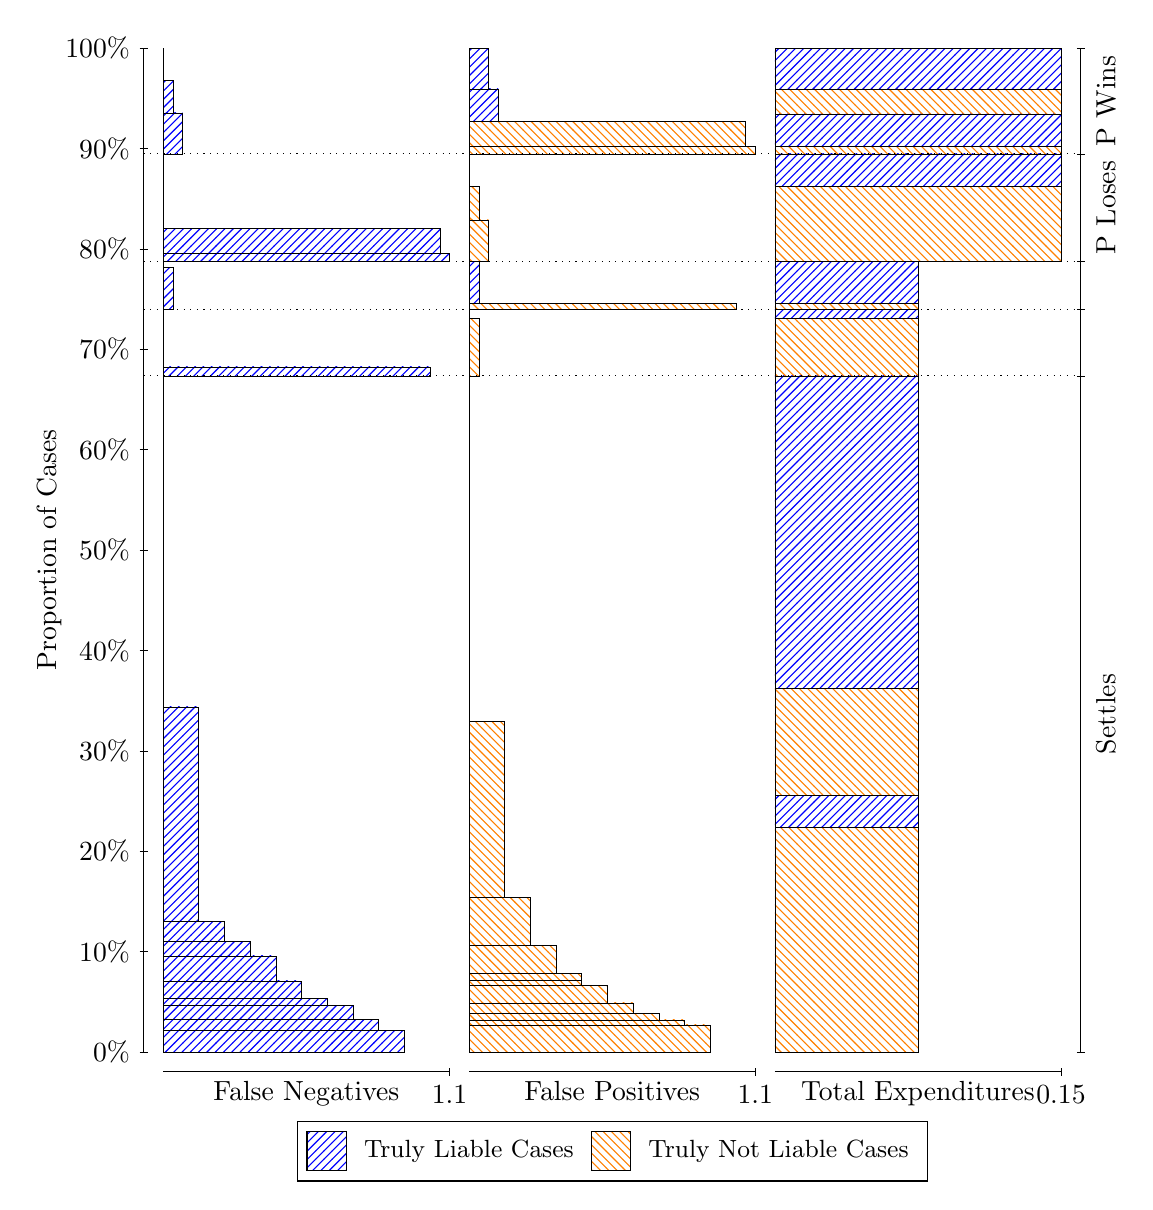
\begin{tikzpicture}
\draw[black, very thin] (1.5,1.75) -- (1.5,14.5);
\node[rotate=90, anchor=center] at (0.3, 8.125) {Proportion of Cases};
\draw[black, very thin] (1.45,1.75) -- (1.55,1.75);
\node[anchor=east] at (1.45, 1.75) {0\%};
\draw[black, very thin] (1.45,3.025) -- (1.55,3.025);
\node[anchor=east] at (1.45, 3.025) {10\%};
\draw[black, very thin] (1.45,4.3) -- (1.55,4.3);
\node[anchor=east] at (1.45, 4.3) {20\%};
\draw[black, very thin] (1.45,5.575) -- (1.55,5.575);
\node[anchor=east] at (1.45, 5.575) {30\%};
\draw[black, very thin] (1.45,6.85) -- (1.55,6.85);
\node[anchor=east] at (1.45, 6.85) {40\%};
\draw[black, very thin] (1.45,8.125) -- (1.55,8.125);
\node[anchor=east] at (1.45, 8.125) {50\%};
\draw[black, very thin] (1.45,9.4) -- (1.55,9.4);
\node[anchor=east] at (1.45, 9.4) {60\%};
\draw[black, very thin] (1.45,10.675) -- (1.55,10.675);
\node[anchor=east] at (1.45, 10.675) {70\%};
\draw[black, very thin] (1.45,11.95) -- (1.55,11.95);
\node[anchor=east] at (1.45, 11.95) {80\%};
\draw[black, very thin] (1.45,13.225) -- (1.55,13.225);
\node[anchor=east] at (1.45, 13.225) {90\%};
\draw[black, very thin] (1.45,14.5) -- (1.55,14.5);
\node[anchor=east] at (1.45, 14.5) {100\%};

\draw[black, very thin] (13.4,1.75) -- (13.4,14.5);
\draw[black, very thin] (13.35,1.75) -- (13.45,1.75);
\node[anchor=west] at (13.35, 1.75) {};
\draw[black, very thin] (13.35,10.336) -- (13.45,10.336);
\node[anchor=west] at (13.35, 10.336) {};
\draw[black, very thin] (13.35,11.179) -- (13.45,11.179);
\node[anchor=west] at (13.35, 11.179) {};
\draw[black, very thin] (13.35,11.793) -- (13.45,11.793);
\node[anchor=west] at (13.35, 11.793) {};
\draw[black, very thin] (13.35,13.157) -- (13.45,13.157);
\node[anchor=west] at (13.35, 13.157) {};
\draw[black, very thin] (13.35,14.5) -- (13.45,14.5);
\node[anchor=west] at (13.35, 14.5) {};

\draw[black, very thin, pattern color=blue, pattern=north east lines] (1.75,1.75) rectangle (4.8118,2.0219);
\draw[black, very thin, pattern color=blue, pattern=north east lines] (1.75,2.0219) rectangle (4.4852,2.1617);
\draw[black, very thin, pattern color=blue, pattern=north east lines] (1.75,2.1617) rectangle (4.1586,2.3388);
\draw[black, very thin, pattern color=blue, pattern=north east lines] (1.75,2.3388) rectangle (3.832,2.4332);
\draw[black, very thin, pattern color=blue, pattern=north east lines] (1.75,2.4332) rectangle (3.5054,2.6531);
\draw[black, very thin, pattern color=blue, pattern=north east lines] (1.75,2.6531) rectangle (3.1788,2.9693);
\draw[black, very thin, pattern color=blue, pattern=north east lines] (1.75,2.9693) rectangle (2.8522,3.1555);
\draw[black, very thin, pattern color=blue, pattern=north east lines] (1.75,3.1555) rectangle (2.5257,3.4077);
\draw[black, very thin, pattern color=blue, pattern=north east lines] (1.75,3.4077) rectangle (2.1991,6.1331);
\draw[black, very thin, pattern color=orange, pattern=north west lines] (1.75,6.1331) rectangle (1.75,10.336);
\draw[black, very thin, pattern color=blue, pattern=north east lines] (1.75,10.336) rectangle (5.1384,10.451);
\draw[black, very thin, pattern color=orange, pattern=north west lines] (1.75,10.451) rectangle (1.75,11.179);
\draw[black, very thin, pattern color=blue, pattern=north east lines] (1.75,11.179) rectangle (1.8725,11.712);
\draw[black, very thin, pattern color=orange, pattern=north west lines] (1.75,11.712) rectangle (1.75,11.793);
\draw[black, very thin, pattern color=blue, pattern=north east lines] (1.75,11.793) rectangle (5.3833,11.89);
\draw[black, very thin, pattern color=blue, pattern=north east lines] (1.75,11.89) rectangle (5.2609,12.208);
\draw[black, very thin, pattern color=orange, pattern=north west lines] (1.75,12.208) rectangle (1.75,13.157);
\draw[black, very thin, pattern color=blue, pattern=north east lines] (1.75,13.157) rectangle (1.9949,13.675);
\draw[black, very thin, pattern color=blue, pattern=north east lines] (1.75,13.675) rectangle (1.8725,14.085);
\draw[black, very thin, pattern color=orange, pattern=north west lines] (1.75,14.085) rectangle (1.75,14.5);
\draw[black, very thin, pattern color=orange, pattern=north west lines] (5.6333,1.75) rectangle (8.6951,2.0952);
\draw[black, very thin, pattern color=orange, pattern=north west lines] (5.6333,2.0952) rectangle (8.3685,2.1576);
\draw[black, very thin, pattern color=orange, pattern=north west lines] (5.6333,2.1576) rectangle (8.0419,2.2354);
\draw[black, very thin, pattern color=orange, pattern=north west lines] (5.6333,2.2354) rectangle (7.7154,2.3748);
\draw[black, very thin, pattern color=orange, pattern=north west lines] (5.6333,2.3748) rectangle (7.3888,2.5946);
\draw[black, very thin, pattern color=orange, pattern=north west lines] (5.6333,2.5946) rectangle (7.0622,2.6572);
\draw[black, very thin, pattern color=orange, pattern=north west lines] (5.6333,2.6572) rectangle (7.0622,2.7479);
\draw[black, very thin, pattern color=orange, pattern=north west lines] (5.6333,2.7479) rectangle (6.7356,3.1031);
\draw[black, very thin, pattern color=orange, pattern=north west lines] (5.6333,3.1031) rectangle (6.409,3.7139);
\draw[black, very thin, pattern color=orange, pattern=north west lines] (5.6333,3.7139) rectangle (6.0824,5.9528);
\draw[black, very thin, pattern color=blue, pattern=north east lines] (5.6333,5.9528) rectangle (5.6333,10.336);
\draw[black, very thin, pattern color=orange, pattern=north west lines] (5.6333,10.336) rectangle (5.7558,11.064);
\draw[black, very thin, pattern color=blue, pattern=north east lines] (5.6333,11.064) rectangle (5.6333,11.179);
\draw[black, very thin, pattern color=orange, pattern=north west lines] (5.6333,11.179) rectangle (9.0217,11.26);
\draw[black, very thin, pattern color=blue, pattern=north east lines] (5.6333,11.26) rectangle (5.7558,11.793);
\draw[black, very thin, pattern color=orange, pattern=north west lines] (5.6333,11.793) rectangle (5.8783,12.316);
\draw[black, very thin, pattern color=orange, pattern=north west lines] (5.6333,12.316) rectangle (5.7558,12.742);
\draw[black, very thin, pattern color=blue, pattern=north east lines] (5.6333,12.742) rectangle (5.6333,13.157);
\draw[black, very thin, pattern color=orange, pattern=north west lines] (5.6333,13.157) rectangle (9.2667,13.253);
\draw[black, very thin, pattern color=orange, pattern=north west lines] (5.6333,13.253) rectangle (9.1442,13.571);
\draw[black, very thin, pattern color=blue, pattern=north east lines] (5.6333,13.571) rectangle (6.0007,13.981);
\draw[black, very thin, pattern color=blue, pattern=north east lines] (5.6333,13.981) rectangle (5.8783,14.5);
\draw[black, very thin, pattern color=orange, pattern=north west lines] (9.5167,1.75) rectangle (11.333,4.5997);
\draw[black, very thin, pattern color=blue, pattern=north east lines] (9.5167,4.5997) rectangle (11.333,5.0114);
\draw[black, very thin, pattern color=orange, pattern=north west lines] (9.5167,5.0114) rectangle (11.333,6.3645);
\draw[black, very thin, pattern color=blue, pattern=north east lines] (9.5167,6.3645) rectangle (11.333,10.336);
\draw[black, very thin, pattern color=orange, pattern=north west lines] (9.5167,10.336) rectangle (11.333,11.064);
\draw[black, very thin, pattern color=blue, pattern=north east lines] (9.5167,11.064) rectangle (11.333,11.179);
\draw[black, very thin, pattern color=orange, pattern=north west lines] (9.5167,11.179) rectangle (11.333,11.26);
\draw[black, very thin, pattern color=blue, pattern=north east lines] (9.5167,11.26) rectangle (11.333,11.793);
\draw[black, very thin, pattern color=orange, pattern=north west lines] (9.5167,11.793) rectangle (13.15,12.742);
\draw[black, very thin, pattern color=blue, pattern=north east lines] (9.5167,12.742) rectangle (13.15,13.157);
\draw[black, very thin, pattern color=orange, pattern=north west lines] (9.5167,13.157) rectangle (13.15,13.253);
\draw[black, very thin, pattern color=blue, pattern=north east lines] (9.5167,13.253) rectangle (13.15,13.663);
\draw[black, very thin, pattern color=orange, pattern=north west lines] (9.5167,13.663) rectangle (13.15,13.981);
\draw[black, very thin, pattern color=blue, pattern=north east lines] (9.5167,13.981) rectangle (13.15,14.5);
\draw[black, dotted] (1.5,10.336) -- (13.4,10.336);
\draw[black, dotted] (1.5,11.179) -- (13.4,11.179);
\draw[black, dotted] (1.5,11.793) -- (13.4,11.793);
\draw[black, dotted] (1.5,13.157) -- (13.4,13.157);
\draw[black, very thin] (1.75,1.5) -- (5.3833,1.5);
\node[anchor=north] at (3.5667, 1.5) {False Negatives};
\draw[black, very thin] (5.3833,1.45) -- (5.3833,1.55);
\node[anchor=north] at (5.3833, 1.45) {1.1};

\draw[black, very thin] (5.6333,1.5) -- (9.2667,1.5);
\node[anchor=north] at (7.45, 1.5) {False Positives};
\draw[black, very thin] (9.2667,1.45) -- (9.2667,1.55);
\node[anchor=north] at (9.2667, 1.45) {1.1};

\draw[black, very thin] (9.5167,1.5) -- (13.15,1.5);
\node[anchor=north] at (11.333, 1.5) {Total Expenditures};
\draw[black, very thin] (13.15,1.45) -- (13.15,1.55);
\node[anchor=north] at (13.15, 1.45) {0.15};

\node[black, centered, rotate=90] at (13.72, 6.0429) {Settles};


\node[black, centered, rotate=90] at (13.72, 12.475) {P Loses};
\node[black, centered, rotate=90] at (13.72, 13.828) {P Wins};

\draw (7.449999999999999,1.5) node[draw=none] (baseCoordinate) {};
\begin{scope}[align=center]
        \matrix[scale=0.5, draw=black, below=0.5cm of baseCoordinate, nodes={draw}, column sep=0.1cm]{
            \node[rectangle, draw, minimum width=0.5cm, minimum height=0.5cm, pattern=north east lines, pattern color=blue] {}; &
            \node[draw=none, font=\small] (B) {Truly Liable Cases}; &
            \node[rectangle, draw, minimum width=0.5cm, minimum height=0.5cm, pattern=north west lines, pattern color=orange] {}; &
            \node[draw=none, font=\small] (B) {Truly Not Liable Cases}; \\
            };
\end{scope}

\end{tikzpicture}
\end{document}